\documentclass[11pt]{article}
\usepackage{myz310e-notes}
\hypersetup{pdftitle={Linear regression and regularisation: least squares, ridge and lasso},pdfauthor={Emre Onur Kahya},pdfsubject={MYZ 310E Machine Learning in Physics, Fall 2026, lecture note 8 (week 4)}}
\newcommand{\Xt}{\tilde X}
\newcommand{\xt}{\tilde{\x}}
\newcommand{\w}{\vect{w}}
\newcommand{\y}{\vect{y}}
\newcommand{\Ic}{D}
\newcommand{\soft}{\operatorname{S}}
\newcommand{\vr}{\vect{r}}
\usepackage{needspace}

\begin{document}
\NoteTitle{8}{4}{Linear regression and regularisation:\\ least squares, ridge and lasso}{Linear regression}{%
Linear regression is the simplest model that is learned by empirical risk minimisation, and the affine map it fits is
the one computed inside every neuron of a standard neural network. This note derives the least-squares solution step by step --- first for a
line through a handful of points, then in matrix form --- and explains its geometry, its algorithms and their cost. It
shows when least squares becomes unstable and introduces the two classical regularisers, ridge ($L_2$) and lasso
($L_1$), with their solutions, their costs and their Bayesian reading, each with a small example that can be redone by
hand. Linear probes of language-model activations and the sparse discovery of
physical laws illustrate how much this small model still does.}

\section{The model}\label{sec:model}

A linear (strictly, affine) regressor predicts
\[
  f_\theta(\x) = \w\T\x + b = w_1 x_1 + \dots + w_d x_d + b, \qquad \theta = (\w, b),\ \w \in \R^d,\ b \in \R .
\]
Each weight is a sensitivity, $w_j = \partial f/\partial x_j$: the change in the prediction when $x_j$ grows by one
unit with the other inputs held fixed. The offset $b$ is the prediction at $\x = \vect{0}$; a neural network would call
this model one neuron with no activation function, and $b$ its bias. We use the
notation of Note~1, Section~2: $n$ training pairs $(\x_i, y_i)$, the inputs stacked as the rows of the $n \times d$ design
matrix $X$, the targets collected in $\y \in \R^n$.

\subsection{The bias trick}\label{sec:biastrick}

The bias complicates every formula by a separate term. It is a good habit to absorb it by prepending a constant
feature: with
\[
  \xt = (x_0, x_1, \dots, x_d)\T \in \R^{d+1}, \qquad \tilde{\w} = (w_0, w_1, \dots, w_d)\T \in \R^{d+1},
  \qquad x_0 = 1,\ w_0 = b,
\]
so that index $0$ always refers to the bias, and we have $\tilde{\w}\T\xt = b \cdot 1 + w_1 x_1 + \dots + w_d x_d = f(\x)$: an affine function of $\x$ is a linear
function of $\xt$. Stacking the $\xt_i\T$ as rows gives the $n \times (d+1)$ matrix $\Xt = [\,\vect{1} \;\; X\,]$, the
design matrix with a column of ones in front, and all $n$ predictions at once are the matrix--vector product
$\Xt\tilde{\w}$. For the five cart positions of the first worked example in Section~\ref{sec:line}, with inputs $x = 0, 1, 2, 3, 4$,
\[
  \Xt = \begin{pmatrix} 1 & 1 & 1 & 1 & 1 \\ 0 & 1 & 2 & 3 & 4 \end{pmatrix}\T, \qquad
  \Xt \begin{pmatrix} b \\ w \end{pmatrix} = \begin{pmatrix} b \\ b + w \\ b + 2w \\ b + 3w \\ b + 4w \end{pmatrix}.
\]
To lighten the formulas we drop the tilde on $\tilde{\w}$: whenever $\w$ multiplies $\Xt$ or $\xt$ it is the full
$(d+1)$-vector $(b, w_1, \dots, w_d)$; from Section~\ref{sec:centring} on, where the bias is split off again, $\w$
multiplying $X$ or $\x$ means the $d$ weights alone. The price of the trick is that the bias is now an ordinary weight;
when we want to treat it differently --- not penalising it in ridge regression, Section~\ref{sec:ridge} --- we have to say
so explicitly.

\paragraph{The neuron picture} Drawn as a network (below), the model has one input node per feature plus a node that
always outputs $1$, and a single output node that forms the weighted sum of its inputs. The weights label the edges
(the ``synaptic strengths'' of the neural vocabulary), and the bias is simply the weight on the constant node --- the
bias trick in pictures. The perceptron and the logistic neuron of Note~9 add a non-linear output to the same picture,
and the networks of week~5 stack many such units.
\begin{center}
\begin{tikzpicture}[x=1cm,y=1cm,font=\small,
  nd/.style={circle,draw,minimum size=6.5mm,inner sep=0pt}]
  \node[nd,fill=gray!15] (c) at (0,1.7) {$1$};
  \node[nd] (a) at (0,0.75) {$x_1$};
  \node at (0,0.05) {$\vdots$};
  \node[nd] (d) at (0,-0.75) {$x_d$};
  \node[nd,minimum size=8mm] (o) at (3.2,0.5) {$\Sigma$};
  \draw[-{Stealth}] (c) -- node[above,sloped,pos=0.3] {$b$} (o);
  \draw[-{Stealth}] (a) -- node[above,sloped,pos=0.3] {$w_1$} (o);
  \draw[-{Stealth}] (d) -- node[below,sloped,pos=0.3] {$w_d$} (o);
  \draw[-{Stealth}] (o) -- (4.6,0.5) node[right] {$f(\x) = b + \w\T\x$};
\end{tikzpicture}
\end{center}

\paragraph{Linear in the parameters} The model is linear in its \emph{parameters}, not necessarily in the original
measurements: $\x$ may contain logarithms, products or powers of raw quantities. Polynomial regression (the polynomial
fits of Note~4, Section~5) is linear regression on the features $(x, x^2, \dots, x^p)$, and everything in this note
applies to it unchanged; Note~10, Section~2, develops such feature maps systematically, and its later sections show how
kernels make them implicit. Categorical inputs enter through the one-hot codes of Note~1, Section~3: the weight of
each category is then the shift of the prediction for examples in that category. With a bias column, one category must
be dropped (or a ridge penalty used), because the $K$ one-hot columns of an attribute sum to the column of ones and
make $\Xt\T\Xt$ singular (Section~\ref{sec:unstable}). Transforming the \emph{target} also changes the noise model: least
squares on $\log y$ assumes additive Gaussian noise of constant size on $\log y$, that is, a roughly constant
\emph{relative} error on $y$ itself.

\section{Least squares}\label{sec:ls}

In the language of Note~4, Sections~1 and~3, a learning algorithm needs a family of models and a loss; linear
regression takes the affine family of Section~\ref{sec:model} and the squared loss of Note~1, Table~2, and empirical
risk minimisation then means minimising the training loss. With the squared loss the empirical risk (up to the factor
$1/n$) is
\[
  J(\w) = \sum_{i=1}^n (\w\T\xt_i - y_i)^2 = \norm{\Xt\w - \y}^2 .
\]
Minimising it is the method of \emph{least squares}. We first solve it for a single input with nothing but ordinary
derivatives, then in matrix form for any $d$.

\subsection{A line through points}\label{sec:line}

For one input the objective is a function of two numbers,
\[
  J(b, w) = \sum_{i=1}^n (y_i - b - w x_i)^2 .
\]
It is a quadratic bowl in $(b, w)$, so its minimum is where both partial derivatives vanish. By the chain rule,
\begin{align*}
  \frac{\partial J}{\partial b} &= -2 \sum_{i=1}^n (y_i - b - w x_i) = 0
    \quad\Longrightarrow\quad n\bar y - n b - n w \bar x = 0
    \quad\Longrightarrow\quad b = \bar y - w \bar x , \\
  \frac{\partial J}{\partial w} &= -2 \sum_{i=1}^n x_i (y_i - b - w x_i) = 0 ,
\end{align*}
with $\bar x = \frac1n\sum_i x_i$ and $\bar y = \frac1n\sum_i y_i$. The first condition says that the best line passes
through the centre of mass $(\bar x, \bar y)$ of the data. Substituting $b = \bar y - w\bar x$ into the second condition
gives $\sum_i x_i\big[(y_i - \bar y) - w(x_i - \bar x)\big] = 0$. The bracket sums to zero over $i$, because
$\sum_i (y_i - \bar y) = \sum_i (x_i - \bar x) = 0$; hence $\bar x$ times the bracket also sums to zero. Subtracting this
zero sum from the condition replaces the factor $x_i$ by $x_i - \bar x$:
\[
  \sum_i (x_i - \bar x)\big[(y_i - \bar y) - w(x_i - \bar x)\big] = S_{xy} - w\,S_{xx} = 0,
  \qquad S_{xy} = \sum_i (x_i - \bar x)(y_i - \bar y),\quad S_{xx} = \sum_i (x_i - \bar x)^2 ,
\]
and therefore
\begin{equation}\label{eq:slope}
  \hat w = \frac{\sum_i (x_i - \bar x)(y_i - \bar y)}{\sum_i (x_i - \bar x)^2} = \frac{S_{xy}}{S_{xx}}
         = \frac{\widehat{\Cov}(x, y)}{\widehat{\Var}(x)}, \qquad \hat b = \bar y - \hat w \bar x .
\end{equation}
The slope is the sample covariance of input and target divided by the sample variance of the input (whether both are
normalised by $1/n$ or by $1/(n-1)$, the factor cancels in the ratio). A convenient
measure of fit is the \emph{coefficient of determination}
\[
  R^2 = 1 - \frac{\sum_i (y_i - \hat y_i)^2}{\sum_i (y_i - \bar y)^2} ,
\]
the fraction of the variance of the targets that the line explains (Section~\ref{sec:geometry} shows why): $R^2 = 1$
for a perfect fit, $R^2 = 0$ for a line no better than the constant $\bar y$. It measures fit on the training data only;
generalisation must still be checked on held-out data (Note~4, Section~4). On held-out data the same formula is used
with the held-out targets and their mean; there it can even be negative, when the model predicts worse than that
constant.

\begin{worked}{fitting a line by hand}
A cart on an air track is photographed once per second. Its positions (cm) at times $x = 0, 1, 2, 3, 4$\,s are
$y = 1, 3, 4, 7, 10$. Here $\bar x = 2$ and $\bar y = 5$; the table collects the centred values.
\begin{center}\small
\begin{tabular}{rrrrrrrr}
\toprule
$x_i$ & $y_i$ & $x_i - \bar x$ & $y_i - \bar y$ & $(x_i - \bar x)(y_i - \bar y)$ & $(x_i - \bar x)^2$ & $\hat y_i$ & $y_i - \hat y_i$ \\
\midrule
0 & 1 & $-2$ & $-4$ & 8 & 4 & 0.6 & 0.4 \\
1 & 3 & $-1$ & $-2$ & 2 & 1 & 2.8 & 0.2 \\
2 & 4 & 0 & $-1$ & 0 & 0 & 5.0 & $-1.0$ \\
3 & 7 & 1 & 2 & 2 & 1 & 7.2 & $-0.2$ \\
4 & 10 & 2 & 5 & 10 & 4 & 9.4 & 0.6 \\
\midrule
 & & & & $S_{xy} = 22$ & $S_{xx} = 10$ & & sum $= 0$ \\
\bottomrule
\end{tabular}
\end{center}
Hence $\hat w = 22/10 = 2.2$\,cm/s (the velocity) and $\hat b = 5 - 2.2 \times 2 = 0.6$\,cm (the initial position). The
residuals sum to zero, as the condition $\partial J/\partial b = 0$ demands. The residual sum of squares is
$0.16 + 0.04 + 1 + 0.04 + 0.36 = 1.6$ and the total sum of squares $\sum_i (y_i - \bar y)^2 = 16 + 4 + 1 + 4 + 25 = 50$,
so $R^2 = 1 - 1.6/50 = 0.968$. Figure~\ref{fig:linefit} (left) shows the line and the residuals.
\end{worked}

\begin{figure}[htbp]
\centering
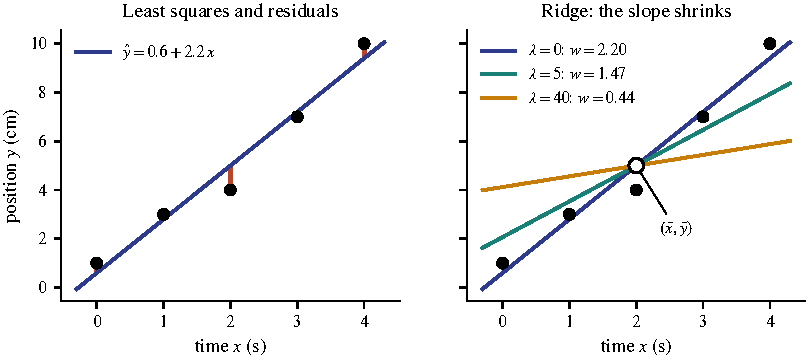
\includegraphics[width=0.94\linewidth]{figures/n8_line_fit.pdf}
\caption{Left: the least-squares line of the cart example (Section~\ref{sec:line}); the vertical segments are the residuals whose
squares are summed. Right: ridge regression on the same data (worked example in Section~\ref{sec:ridgeclosed}). As $\lambda$ grows the
slope shrinks towards zero; with the bias unpenalised, every line still passes through $(\bar x, \bar y) = (2, 5)$.}
\label{fig:linefit}
\end{figure}

\begin{algorithm}[htbp]
\caption{Simple linear regression (one input)}
\label{alg:simple}
\begin{algorithmic}[1]
\Require pairs $(x_i, y_i)$, $i = 1, \dots, n$
\Ensure intercept $\hat b$ and slope $\hat w$
\State $\bar x \gets \frac1n\sum_i x_i$, \quad $\bar y \gets \frac1n\sum_i y_i$ \Comment{first pass}
\State $S_{xy} \gets \sum_i (x_i - \bar x)(y_i - \bar y)$, \quad $S_{xx} \gets \sum_i (x_i - \bar x)^2$ \Comment{second pass}
\State $\hat w \gets S_{xy}/S_{xx}$ \Comment{requires at least two distinct $x_i$}
\State $\hat b \gets \bar y - \hat w\bar x$
\State \Return $(\hat b, \hat w)$; predict with $\hat y = \hat b + \hat w x$
\end{algorithmic}
\end{algorithm}

\begin{runtime}{simple linear regression (Algorithm~\ref{alg:simple})}
Training $O(n)$: two passes, constant work per point. Prediction $O(1)$ per query; memory $O(1)$. Centring first
avoids the one-pass formula $S_{xy} = \sum x_i y_i - n\bar x\bar y$, which loses digits when the data sit far from $0$.
\end{runtime}

\subsection{The gradient in matrix form}\label{sec:matrixgrad}

For $d$ inputs we repeat the calculation with vectors. Two rules of matrix calculus suffice. For a fixed vector
$\vect{a}$ and a fixed symmetric matrix $A$,
\[
  \nabla_{\w}\,(\vect{a}\T\w) = \vect{a}, \qquad \nabla_{\w}\,(\w\T A\w) = 2A\w .
\]
Both follow from partial derivatives: $\partial(\sum_j a_j w_j)/\partial w_k = a_k$, and
$\partial(\sum_{i,j} w_i A_{ij} w_j)/\partial w_k = \sum_j A_{kj} w_j + \sum_i w_i A_{ik} = 2(A\w)_k$ when $A = A\T$.
Now expand the square, using $(\Xt\w)\T\y = \y\T\Xt\w$ (a scalar equals its transpose):
\[
  J(\w) = (\Xt\w - \y)\T(\Xt\w - \y) = \w\T(\Xt\T\Xt)\w - 2\,(\Xt\T\y)\T\w + \y\T\y .
\]
The first term is a quadratic form with the symmetric matrix $A = \Xt\T\Xt$, the second is linear with
$\vect{a} = -2\Xt\T\y$, the third is constant. Hence
\[
  \nabla J(\w) = 2\Xt\T\Xt\w - 2\Xt\T\y = 2\Xt\T(\Xt\w - \y), \qquad H = \nabla^2 J = 2\Xt\T\Xt .
\]
The gradient has a direct reading: $\Xt\w - \y$ is the vector of prediction errors, and $\Xt\T$ sums each feature
column weighted by these errors. The Hessian is positive semi-definite, because
$\vect{v}\T\Xt\T\Xt\vect{v} = \norm{\Xt\vect{v}}^2 \ge 0$ for every $\vect{v}$, so $J$ is convex (Note~7, Section~4) and
every stationary point is a global minimum. Setting the gradient to zero gives the \emph{normal equations}
\begin{equation}\label{eq:normal}
  \Xt\T\Xt\, \w = \Xt\T\y, \qquad \hat{\w} = (\Xt\T\Xt)^{-1}\Xt\T\y \quad\text{if } \Xt\T\Xt \text{ is invertible.}
\end{equation}
The $(d+1) \times (d+1)$ matrix $\Xt\T\Xt$ contains the sums $\sum_i \tilde x_{ij}\tilde x_{ik}$ of products of features;
$\Xt\T\y$ contains the sums $\sum_i \tilde x_{ij} y_i$. For $d = 1$, \eqref{eq:normal} reduces to the two conditions of
Section~\ref{sec:line}. Note~2, Section~3, showed that minimising squared error is maximum likelihood under Gaussian
noise, so $\hat{\w}$ is also the maximum-likelihood estimate of that model.

\subsection{Centring removes the bias}\label{sec:centring}

Here, and wherever $\w$ multiplies $X$ or $\x$ rather than $\Xt$ or $\xt$, $\w \in \R^d$ denotes the weights without
the bias, and the full vector is $\tilde{\w} = (b, \w)$ (Section~\ref{sec:biastrick}). The first row of \eqref{eq:normal} belongs to the column of ones and reads
$\sum_i (b + \w\T\x_i - y_i) = 0$, i.e.
\[
  \hat b = \bar y - \hat{\w}\T\bar{\x}, \qquad \bar{\x} = \tfrac1n \textstyle\sum_i \x_i ,
\]
exactly as for the line. Substituting it back, each residual becomes $y_i - b - \w\T\x_i = (y_i - \bar y) -
\w\T(\x_i - \bar{\x})$. So the weights solve the least-squares problem for the \emph{centred} data $X_c$ (rows
$\x_i - \bar{\x}$) and $\y_c$ (entries $y_i - \bar y$), with no bias at all:
\[
  X_c\T X_c\, \hat{\w} = X_c\T \y_c, \qquad \hat b = \bar y - \hat{\w}\T\bar{\x} .
\]
This is the second way of handling the bias: centre, solve a $d \times d$ system, and recover $b$ at the end. It is the
form we use for ridge and lasso, where the bias must not be penalised. When the features are already centred, the
column of ones is orthogonal to the others, $\Xt\T\Xt$ is block diagonal and $\hat b = \bar y$, as in the next example.

\begin{worked}{normal equations with two features}
The output $y$ of a detector channel is recorded at five settings of two control voltages, given as deviations from
their nominal values (so each column has mean zero). We write $\vect{f}_j \in \R^n$ for \emph{column} $j$ of $X$, the
values of feature $j$ over all $n$ examples, to keep it apart from the example $\x_i \in \R^d$, which is \emph{row} $i$:
\[
  \vect{f}_1 = (-2, -1, 0, 1, 2), \quad \vect{f}_2 = (1, -1, -1, 0, 1), \quad \y = (1, 2, 4, 5, 8) .
\]
The sums needed are $n = 5$, $\sum_i x_{i1} = \sum_i x_{i2} = 0$, $\sum_i y_i = 20$, $\norm{\vect{f}_1}^2 = 10$,
$\norm{\vect{f}_2}^2 = 4$, $\vect{f}_1\T\vect{f}_2 = -2 + 1 + 0 + 0 + 2 = 1$, $\vect{f}_1\T\y = -2 - 2 + 0 + 5 + 16
= 17$ and $\vect{f}_2\T\y = 1 - 2 - 4 + 0 + 8 = 3$. The normal equations \eqref{eq:normal} are
\[
  \begin{pmatrix} 5 & 0 & 0 \\ 0 & 10 & 1 \\ 0 & 1 & 4 \end{pmatrix}
  \begin{pmatrix} b \\ w_1 \\ w_2 \end{pmatrix} = \begin{pmatrix} 20 \\ 17 \\ 3 \end{pmatrix}.
\]
The first row gives $b = 4 = \bar y$. The remaining $2 \times 2$ system has determinant $10 \cdot 4 - 1 \cdot 1 = 39$ and
\[
  \begin{pmatrix} w_1 \\ w_2 \end{pmatrix} = \frac{1}{39}\begin{pmatrix} 4 & -1 \\ -1 & 10 \end{pmatrix}
  \begin{pmatrix} 17 \\ 3 \end{pmatrix} = \frac{1}{39}\begin{pmatrix} 65 \\ 13 \end{pmatrix}
  = \begin{pmatrix} 5/3 \\ 1/3 \end{pmatrix} \approx \begin{pmatrix} 1.667 \\ 0.333 \end{pmatrix}.
\]
The fitted values $\hat y = 4 + \tfrac53 x_1 + \tfrac13 x_2$ are $(1, 2, 3.667, 5.667, 7.667)$ and the residuals
$\vr = \y - \hat{\y} = (0, 0, \tfrac13, -\tfrac23, \tfrac13)$. Check: $\sum_i r_i = 0$, $\vect{f}_1\T\vr = -\tfrac23 +
\tfrac23 = 0$ and $\vect{f}_2\T\vr = -\tfrac13 + \tfrac13 = 0$ --- the residual is orthogonal to all three columns, as the
next subsection explains. \texttt{np.linalg.lstsq} returns the same $(4, 1.667, 0.333)$.
\end{worked}

\subsection{Geometry: an orthogonal projection}\label{sec:geometry}

The fitted values $\hat{\y} = \Xt\hat{\w}$ lie in the column space of $\Xt$, the set of all predictions the model can make
(a subspace of $\R^n$ of dimension $d+1$ when the columns are independent, less otherwise). The normal equations say $\Xt\T(\y - \hat{\y}) = \vect{0}$: the residual is
orthogonal to every column, so $\hat{\y}$ is the orthogonal projection of $\y$ onto that space, the closest point to the
observations. In matrix form $\hat{\y} = P\y$ with the projection (``hat'') matrix $P = \Xt(\Xt\T\Xt)^{-1}\Xt\T$, which
satisfies $P^2 = P$: projecting twice changes nothing. Two consequences are worth remembering. With a constant column,
the residuals sum to zero. And $R^2$ is a Pythagoras theorem: write the centred targets $\y_c = \y - \bar y\vect{1}$ as
\[
  \y - \bar y\vect{1} = (\hat{\y} - \bar y\vect{1}) + (\y - \hat{\y}) .
\]
The first vector lies in the column space (both $\hat{\y}$ and $\vect{1}$ do, since $\vect{1}$ is a column of $\Xt$); the
second is the residual, orthogonal to that space. The two are perpendicular, so
$\norm{\y_c}^2 = \norm{\hat{\y} - \bar y\vect{1}}^2 + \norm{\y - \hat{\y}}^2$: the total sum of squares equals the
\emph{explained} sum of squares (the spread of the fitted values about $\bar y$) plus the residual sum of squares. Hence
$R^2 = 1 - \text{residual}/\text{total} = \text{explained}/\text{total}$ lies between 0 and 1 for least squares with a
bias. In the detector example: $30 = 29.33 + 0.67$, so $R^2 = 0.978$.

\subsection{Computing the solution}\label{sec:computing}

\paragraph{Normal equations, but not the inverse} Never form the inverse in \eqref{eq:normal}. The matrix $\Xt\T\Xt$ is
symmetric and (if the columns are independent) positive definite, so the system is solved by a Cholesky factorisation
$\Xt\T\Xt = LL\T$ and two triangular solves (Algorithm~\ref{alg:normal}). This is the fastest exact method and can be
accumulated in one pass over data that do not fit in memory, since $\Xt\T\Xt = \sum_i \xt_i\xt_i\T$ and
$\Xt\T\y = \sum_i y_i\xt_i$.

\paragraph{QR or SVD} The weakness of the normal equations is numerical. Every $n \times p$ matrix ($n \ge p$) can be
factorised as $\Xt = USV\T$, the (thin) \emph{singular value decomposition}: $U \in \R^{n \times p}$ and
$V \in \R^{p \times p}$ have orthonormal columns and $S$ is diagonal with entries $s_1 \ge s_2 \ge \dots \ge 0$, the
\emph{singular values}. The $s_j^2$ are the eigenvalues of $\Xt\T\Xt$ and the columns of $V$ (the right singular
vectors) its eigenvectors; Section~\ref{sec:svd} uses this in detail. The condition number $\kappa$ of a matrix (ratio
of largest to smallest singular value) measures how much relative errors are amplified; forming $\Xt\T\Xt$ squares it,
$\kappa(\Xt\T\Xt) = \kappa(\Xt)^2$, and loses about twice as many significant digits. Factorising $\Xt = QR$ with $Q$
having orthonormal columns and $R$ upper triangular avoids the squaring. Substituting, $\Xt\T\Xt = R\T Q\T Q R = R\T R$
because $Q\T Q = I$, and $\Xt\T\y = R\T Q\T\y$, so \eqref{eq:normal} becomes $R\T R\w = R\T Q\T\y$. When the columns
are independent, $R\T$ is invertible and may be cancelled, leaving the triangular system $R\w = Q\T\y$
(Algorithm~\ref{alg:qr}). Library routines such as \texttt{np.linalg.lstsq} use the SVD instead (LAPACK's
\texttt{gelsd}): substituting $\Xt = USV\T$ in the same way gives $\hat{\w} = V\,\mathrm{diag}(1/s_j)\,U\T\y$, where
singular values below a small tolerance are dropped rather than inverted (Algorithm~\ref{alg:svdls}). This costs a few
times more than QR but also copes with rank-deficient $\Xt$, where it returns the solution of smallest norm
(Section~\ref{sec:unstable}).

\begin{algorithm}[htbp]
\caption{Least squares by the normal equations (Cholesky)}
\label{alg:normal}
\begin{algorithmic}[1]
\Require design matrix $\Xt \in \R^{n \times p}$ (with the column of ones, $p = d+1$), targets $\y \in \R^n$
\Ensure weights $\hat{\w} \in \R^p$
\State $G \gets \Xt\T\Xt$ \Comment{$p \times p$ Gram matrix, $O(np^2)$}
\State $\vect{c} \gets \Xt\T\y$ \Comment{$O(np)$}
\State $L \gets \Call{Cholesky}{G}$ \Comment{$G = LL\T$, $L$ lower triangular, $O(p^3)$}
\State solve $L\vect{z} = \vect{c}$ by forward substitution, then $L\T\hat{\w} = \vect{z}$ by back substitution \Comment{$O(p^2)$}
\State \Return $\hat{\w}$; predict with $\hat y = \hat{\w}\T\xt$
\end{algorithmic}
\end{algorithm}

\begin{algorithm}[htbp]
\caption{Least squares by Householder QR factorisation}
\label{alg:qr}
\begin{algorithmic}[1]
\Require $\Xt \in \R^{n \times p}$ with independent columns, $\y \in \R^n$
\Ensure weights $\hat{\w}$
\State $(Q, R) \gets \Call{HouseholderQR}{\Xt}$ \Comment{$Q \in \R^{n \times p}$, $Q\T Q = I$, $R$ upper triangular, $O(np^2)$}
\State $\vect{c} \gets Q\T\y$ \Comment{$O(np)$}
\State solve $R\hat{\w} = \vect{c}$ by back substitution \Comment{$O(p^2)$}
\State \Return $\hat{\w}$ \Comment{residual sum of squares: $\norm{\y}^2 - \norm{\vect{c}}^2$, see below}
\end{algorithmic}
\end{algorithm}

\begin{algorithm}[htbp]
\caption{Least squares by the thin SVD (minimum-norm solution, as in \texttt{lstsq})}
\label{alg:svdls}
\begin{algorithmic}[1]
\Require $\Xt \in \R^{n \times p}$ (any rank), $\y \in \R^n$, relative tolerance $\tau$ (e.g.\ $10^{-12}$)
\Ensure the minimum-norm minimiser $\hat{\w}$ of $\norm{\Xt\w - \y}^2$
\State $(U, \vect{s}, V) \gets \Call{ThinSVD}{\Xt}$ \Comment{$r = \min(n, p)$ singular values, $O(np\,r)$}
\State $\vect{c} \gets U\T\y$ \Comment{components of $\y$ along the $\vect{u}_j$, $O(nr)$}
\State $\hat{\w} \gets \sum_{j:\ s_j > \tau s_1} \vect{v}_j\, c_j/s_j$ \Comment{tiny $s_j$ are dropped, not inverted; $O(pr)$}
\State \Return $\hat{\w}$
\end{algorithmic}
\end{algorithm}

In Algorithm~\ref{alg:qr}, the fitted values are $\hat{\y} = Q Q\T\y$, the projection of $\y$ onto the column space, and
$\vect{c} = Q\T\y$ holds its coordinates in the orthonormal basis $Q$; by Pythagoras
$\norm{\y - \hat{\y}}^2 = \norm{\y}^2 - \norm{\hat{\y}}^2 = \norm{\y}^2 - \norm{\vect{c}}^2$, so the residual sum of
squares comes for free. Algorithm~\ref{alg:svdls} works also when $d + 1 > n$ or when columns are dependent: the dropped
directions are exactly those along which the data say nothing, and leaving them at zero gives the solution of smallest
norm.

\begin{runtime}{least squares, direct methods (Algorithms~\ref{alg:normal}, \ref{alg:qr} and~\ref{alg:svdls})}
With $n$ examples and $p = d + 1$ parameters. \emph{Normal equations}: forming $\Xt\T\Xt$ costs $O(np^2)$ (each of the
$p^2$ entries is a sum over $n$ products), $\Xt\T\y$ costs $O(np)$, Cholesky $O(p^3)$ (about $p^3/3$ operations), the
triangular solves $O(p^2)$; total $O(np^2 + p^3)$, usually dominated by $np^2$ because $n > p$. Memory: $O(p^2)$ for the
Gram matrix, and the data may be streamed. \emph{QR}: $O(np^2)$ time (about twice the normal equations), $O(np)$ memory
since the whole matrix is factorised; the SVD has the same order, $O(np\min(n, p))$, with a constant a few times
larger, and $O(np)$ memory. \emph{Prediction}: $O(d)$ per query, one dot
product. \emph{Typical sizes}: $n = 10^6$, $d = 10^3$ means $np^2 \approx 10^{12}$ operations --- seconds to minutes on a
laptop, much less on a GPU, where these dense matrix products run in parallel. For $d \sim 10^5$ (text or genomic
features) the $p^2$ memory ($10^{10}$ numbers) and the $p^3$ time are prohibitive, and iterative methods take over.
\end{runtime}

\paragraph{Gradient descent} The normal equations are the exception, not the rule: they exist only because a linear
model with the squared loss (plus, possibly, an $L_2$ penalty, Section~\ref{sec:ridge}) has a \emph{quadratic}
objective, whose gradient is linear in $\w$. With another loss (the absolute or Huber error, the logistic loss of
Note~9) or a non-linear model, setting the gradient to zero gives equations that cannot be solved in closed form, and
iterative minimisation (Note~7, Section~3) is the general method; the lasso of Section~\ref{sec:lasso} is a first
example. Even for least squares, gradient descent pays off for very large $n$ or $d$, because it needs only
matrix--vector products. It is customary to use the \emph{mean} loss $L(\w) = \frac1n\norm{\Xt\w - \y}^2 = J(\w)/n$, whose size does not
grow with the number of examples. Dividing by $n$ does not move the minimiser; it only rescales the gradient, so the safe
step size depends on which form is used. The update is
\[
  \w \leftarrow \w - \eta\,\nabla L(\w) = \w - \eta\,\tfrac{2}{n}\,\Xt\T(\Xt\w - \y) .
\]
The Hessian of $L$ is the constant matrix $\frac2n\Xt\T\Xt$, so the analysis of Note~7, Section~3, applies exactly: the step must
satisfy $\eta < 2/\mu_{\max}$, with $\mu_{\max}$ the largest eigenvalue of $\frac2n\Xt\T\Xt$, and the number of
iterations grows with its condition number --- one more reason to standardise the features. Mini-batch gradients
(Note~7, Section~5) replace the sum over all $n$ examples by a sum over a random batch of $n'$ and make the method work
on data that do not fit in memory (Algorithm~\ref{alg:gd}).

\begin{worked}{one gradient-descent step}
Take the cart data of Section~\ref{sec:line} with $\theta = (b, w)$, start at $\theta_0 = (0, 0)$ and use
$\eta = 0.05$, minimising the mean loss $L$. At the start all predictions are zero, so the errors are $\Xt\theta_0 - \y = -\y$ and
\[
  \nabla L(\theta_0) = -\tfrac25\,\Xt\T\y = -\tfrac25 \begin{pmatrix} \sum_i y_i \\ \sum_i x_i y_i \end{pmatrix}
  = -\tfrac25\begin{pmatrix} 25 \\ 72 \end{pmatrix} = \begin{pmatrix} -10 \\ -28.8 \end{pmatrix},
\]
with $\sum_i x_i y_i = 0 + 3 + 8 + 21 + 40 = 72$. The step gives $\theta_1 = (0, 0) - 0.05\,(-10, -28.8) = (0.5, 1.44)$,
and the mean squared error falls from $L(\theta_0) = \frac15(1 + 9 + 16 + 49 + 100) = 35$ to $L(\theta_1) = 4.10$; a second
step gives $(0.662, 1.916)$ with $L = 0.74$. The minimum is $L(0.6, 2.2) = 1.6/5 = 0.32$. Is the step size safe? The
Hessian $\frac25\Xt\T\Xt = \frac25\begin{psmallmatrix} 5 & 10 \\ 10 & 30 \end{psmallmatrix} =
\begin{psmallmatrix} 2 & 4 \\ 4 & 12 \end{psmallmatrix}$ has eigenvalues $0.60$ and $13.40$, so any $\eta < 2/13.40 = 0.149$
converges; with $\eta = 0.05$ the iterate agrees with $(0.600, 2.200)$ to three decimals after 200 steps. The condition
number $13.40/0.60 \approx 22$ comes from the uncentred $x$: with $x - \bar x$ the Hessian is $\mathrm{diag}(2, 4)$.

\emph{A stochastic step.} Stochastic gradient descent uses one example at a time, with the gradient
$2(\theta\T\xt_i - y_i)\,\xt_i$ of its own squared error. From $\theta_0 = (0, 0)$ the example $(x, y) = (3, 7)$ gives
$2(0 - 7)(1, 3) = (-14, -42)$ and the step $\theta_1 = (0.7, 2.1)$; the example $(0, 1)$ gives $(0.1, 0)$ and
$(4, 10)$ gives $(1.0, 4.0)$. Each step costs a fifth of the batch step, but its direction depends on which example is
drawn, and the mean squared error after it ranges from $0.35$ to $34.0$. Averaged over the five possible examples the
step is $(0.5, 1.44)$, exactly the batch step: the stochastic gradient is unbiased but noisy (Note~7, Section~5).
\end{worked}

\begin{algorithm}[htbp]
\caption{Least squares by mini-batch stochastic gradient descent}
\label{alg:gd}
\begin{algorithmic}[1]
\Require $\Xt \in \R^{n \times p}$, $\y$, learning rate $\eta$, batch size $n'$, number of epochs $E$, penalty $\lambda' \ge 0$
\Ensure approximate minimiser $\w$ of $L(\w) + \lambda'\sum_{j \ge 1} w_j^2$, with $L(\w) = \frac1n\norm{\Xt\w - \y}^2$
\State $\w \gets \vect{0}$ \Comment{the objective is convex: any start works}
\For{$e = 1, \dots, E$}
  \State shuffle the indices $1, \dots, n$ and cut them into batches $B$ of size $n'$ (the last may be smaller)
  \For{each batch $B$}
    \State $\vect{g} \gets \frac{2}{|B|}\sum_{i \in B} (\w\T\xt_i - y_i)\,\xt_i$ \Comment{$O(n'p)$; $B = \{1,\dots,n\}$ gives batch GD}
    \State $\vect{g} \gets \vect{g} + 2\lambda'\Ic\w$ \Comment{$\Ic = \mathrm{diag}(0, 1, \dots, 1)$; $\lambda' = 0$: least squares}
    \State $\w \gets \w - \eta\,\vect{g}$
  \EndFor
  \State optionally decrease $\eta$; stop when the validation error no longer improves
\EndFor
\State \Return $\w$
\end{algorithmic}
\end{algorithm}

\begin{runtime}{gradient descent for least squares (Algorithm~\ref{alg:gd})}
One full gradient costs two matrix--vector products, $O(np)$; one epoch of mini-batch descent also costs $O(np)$ in total,
split into $n/n'$ cheap steps of $O(n'p)$. Batch gradient descent needs about $\kappa\log(1/\epsilon)$ iterations to reach
accuracy $\epsilon$, with $\kappa$ the condition number of $\Xt\T\Xt$, so its total cost is $O(\kappa\,np\log(1/\epsilon))$
--- no $p^3$ term and no $p \times p$ matrix. Memory: $O(p)$ for the weights plus one batch, $O(n'p)$, so the data can
stream from disk. Prediction: $O(d)$ per query. Gradient descent wins when $p$ is large, the data are sparse (each
product then costs only the number of non-zero entries) or an approximate answer suffices; for moderate $p$ and
ill-conditioned data the direct methods are faster and exact. \emph{Typical sizes}: for $n = 10^8$ and $d = 50$ one epoch
is about $10^{10}$ operations, seconds on a GPU, where each mini-batch step is a pair of dense matrix--vector products
that parallelise well.
\end{runtime}

\paragraph{Other iterative methods} Newton's method (Note~7, Section~6) is exact here: the Hessian $2\Xt\T\Xt$ is
constant, and from \emph{any} $\w$ the Newton step gives
$\w - (2\Xt\T\Xt)^{-1}\,2\Xt\T(\Xt\w - \y) = (\Xt\T\Xt)^{-1}\Xt\T\y$, the solution of the normal equations --- one Newton
step \emph{is} solving them. Between the direct methods and gradient descent sits the \emph{conjugate gradient} method
applied to the normal equations (as in the library routines LSQR or LSMR). Like gradient descent it needs only products
with $\Xt$ and $\Xt\T$, $O(np)$ per iteration and $O(n + p)$ extra memory; it reaches the exact solution in at most $p$
iterations in exact arithmetic, and in practice needs about $\sqrt{\kappa}\log(1/\epsilon)$ iterations instead of the
$\kappa\log(1/\epsilon)$ of gradient descent~\cite{nocedal2006}. Natural-gradient and adaptive methods matter for
non-quadratic objectives and are left to Note~7 and week~5.

\section{When least squares is unstable}\label{sec:unstable}

The solution is unique only if the columns of $\Xt$ are linearly independent, and it is reliable only if they are far
from dependent.

\begin{itemize}
\item \emph{Collinear features.} If two inputs measure almost the same thing, the data cannot tell how to split the
weight between them: $w_1 + w_2$ is well determined, $w_1 - w_2$ is not. Figure~\ref{fig:collinear} shows 300 repetitions
of an experiment with $x_2 = x_1 + $ small noise: least-squares estimates of $w_1$ scatter with a standard deviation of
2.05 around the true value~1, along a line of nearly constant $w_1 + w_2$. Predictions inside the data remain fine;
interpretations and predictions away from the data do not.
\item \emph{More features than examples.} If $d + 1 > n$, $\Xt\T\Xt$ is singular and infinitely many $\w$ fit the training
data exactly: adding to $\hat{\w}$ any vector $\vect{v}$ with $\Xt\vect{v} = \vect{0}$ (there are such vectors when the
$d+1$ columns live in $\R^n$ with $n < d + 1$) changes no prediction. \texttt{lstsq} then returns the solution of minimum
norm --- the implicit preference behind the double-descent curve of Note~4, Section~8.
\end{itemize}

\begin{figure}[htbp]
\centering
\begin{minipage}[c]{0.42\linewidth}
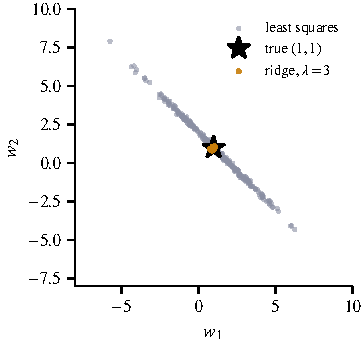
\includegraphics[width=\linewidth]{figures/collinear.pdf}
\end{minipage}\hfill
\begin{minipage}[c]{0.54\linewidth}
\caption{Estimates of $(w_1, w_2)$ from 300 datasets of 30 points with nearly collinear inputs and true weights
$(1, 1)$. Least squares (grey) spreads along the poorly determined direction $w_1 - w_2$; ridge regression with
$\lambda = 3$ (amber) stays close to the truth: standard deviation of $w_1$ falls from 2.05 to 0.05, at the price of a
small bias (mean 0.95).}
\label{fig:collinear}
\end{minipage}
\end{figure}

\begin{worked}{two thermometers}
Two thermometers read almost the same temperature deviation; the two feature columns of four centred readings are
\[
  \vect{f}_1 = (-2, -1, 1, 2), \qquad \vect{f}_2 = (-2, -0.9, 0.9, 2) .
\]
Then $\norm{\vect{f}_1}^2 = 10$, $\norm{\vect{f}_2}^2 = 9.62$, $\vect{f}_1\T\vect{f}_2 = 9.8$, and
$X\T X = \begin{psmallmatrix} 10 & 9.8 \\ 9.8 & 9.62 \end{psmallmatrix}$ has the tiny determinant
$10 \cdot 9.62 - 9.8^2 = 0.16$. Consider two target vectors that differ by $0.1$ in two entries, as two repetitions of
the experiment might. Both inputs and both target vectors are centred (each sums to zero), so by
Section~\ref{sec:centring} the bias is $\bar y = 0$ and only the $2 \times 2$ matrix $X\T X$ is needed:
\begin{center}\small
\begin{tabular}{lccc}
\toprule
 & targets $\y$ & $X\T\y$ & least squares $(\hat w_1, \hat w_2)$ \\
\midrule
data set A & $(-4.1, -1.8, 2.0, 3.9)$ & $(19.8, 19.42)$ & $(1.00, 1.00)$ \\
data set B & $(-4.1, -1.9, 2.1, 3.9)$ & $(20.0, 19.6)$ & $(2.00, 0.00)$ \\
\bottomrule
\end{tabular}
\end{center}
For A, $\hat{\w} = \frac{1}{0.16}\begin{psmallmatrix} 9.62 & -9.8 \\ -9.8 & 10 \end{psmallmatrix}
\begin{psmallmatrix} 19.8 \\ 19.42 \end{psmallmatrix} = \frac{1}{0.16}\begin{psmallmatrix} 0.16 \\ 0.16
\end{psmallmatrix}$; for B the same matrix gives $\frac{1}{0.16}(0.32, 0)$. A change of $0.1$ in the data moves the weights
by $1$: the difference $w_1 - w_2$ jumps from $0$ to $2$, while the sum $w_1 + w_2 = 2$ is the same in both. The singular
values of $X$ are $4.43$ and $0.090$ (the square roots of the eigenvalues $19.61$ and $0.0082$ of $X\T X$), so $\kappa(X) = 49$ and $\kappa(X\T X) \approx 2400$; the right singular vectors
are $(0.714, 0.700)$ (the sum direction) and $(0.700, -0.714)$ (the difference direction). We return to this example
with ridge regression in Section~\ref{sec:ridgeclosed}.
\end{worked}

\section{Ridge regression}\label{sec:ridge}

Regularisation (Note~4, Section~7) adds to the training loss a penalty $\Omega(\w) \ge 0$ that encodes a preference
among parameter values, weighted by $\lambda \ge 0$:
\[
  J_\lambda(\w) = \norm{\Xt\w - \y}^2 + \lambda\,\Omega(\w) .
\]
The choice $\Omega = \sum_j w_j^2$ gives ridge regression (this section), $\Omega = \sum_j |w_j|$ the lasso
(Section~\ref{sec:lasso}) and a mixture of the two the elastic net (Section~\ref{sec:paths}); each $\Omega$ is also a prior
belief about $\w$ (Section~\ref{sec:bayesian}). Ridge regression uses the weight-decay penalty, and was introduced for
regression by Hoerl and Kennard~\cite{hoerl1970}:
\begin{equation}\label{eq:ridge}
  J_\lambda(\w) = \norm{\Xt\w - \y}^2 + \lambda \sum_{j=1}^d w_j^2 ,
\end{equation}
leaving the bias unpenalised: shifting all targets by a constant should shift $b$, not shrink it, and a penalised bias
would make the predictions depend on where we put the origin of $y$~\cite[Section~3.4.1]{hastie2009}.

\subsection{The closed form, step by step}\label{sec:ridgeclosed}

Write the penalty as a quadratic form, $\sum_{j=1}^d w_j^2 = \w\T\Ic\w$, where $\Ic = \mathrm{diag}(0, 1, \dots, 1)$ is
the $(d+1)\times(d+1)$ diagonal matrix that skips the bias entry and keeps the weights. Then
\[
  J_\lambda(\w) = \w\T(\Xt\T\Xt + \lambda\Ic)\w - 2(\Xt\T\y)\T\w + \y\T\y ,
\]
and the two rules of Section~\ref{sec:matrixgrad} give
\[
  \nabla J_\lambda = 2\Xt\T(\Xt\w - \y) + 2\lambda\Ic\w = \vect{0}
  \quad\Longrightarrow\quad
  \hat{\w}_\lambda = (\Xt\T\Xt + \lambda \Ic)^{-1}\Xt\T\y .
\]
The penalty simply adds $\lambda$ to the diagonal of the Gram matrix, except for the bias entry. For $\lambda > 0$ the
matrix is positive definite, so the solution is unique even when $d > n$. To see this, take any
$\vect{v} = (v_0, v_1, \dots, v_d) \neq \vect{0}$, with $v_0$ the bias component; then
$\vect{v}\T(\Xt\T\Xt + \lambda\Ic)\vect{v} = \norm{\Xt\vect{v}}^2 + \lambda\sum_{j \ge 1} v_j^2$. If some $v_j$ with
$j \ge 1$ is non-zero, the second term is positive. Otherwise $\vect{v} = (v_0, 0, \dots, 0)$ with $v_0 \neq 0$, so
$\Xt\vect{v} = v_0\vect{1}$ and $\norm{\Xt\vect{v}}^2 = n v_0^2 > 0$. Because $\Ic$ has a zero in the bias position,
the first equation of $(\Xt\T\Xt + \lambda\Ic)\w = \Xt\T\y$ is the same as in least squares, so with centred data
(Section~\ref{sec:centring}) it again gives $\hat b = \bar y - \hat{\w}\T\bar{\x}$, and the weights are
\begin{equation}\label{eq:ridgec}
  \hat{\w}_\lambda = (X_c\T X_c + \lambda I)^{-1} X_c\T\y_c .
\end{equation}
For a single centred input this is
\[
  \hat w_\lambda = \frac{\sum_i x_i y_i}{\sum_i x_i^2 + \lambda} = \frac{S_{xx}}{S_{xx} + \lambda}\,\hat w_{\mathrm{LS}} ,
\]
the least-squares slope multiplied by a \emph{shrinkage factor} between 0 and 1.

\begin{worked}{ridge shrinkage in one dimension}
For the cart data ($S_{xy} = 22$, $S_{xx} = 10$, $\bar x = 2$, $\bar y = 5$), $\hat w_\lambda = 22/(10 + \lambda)$ and,
since the bias is not penalised, $\hat b_\lambda = 5 - 2\hat w_\lambda$:
\begin{center}\small
\begin{tabular}{lccccc}
\toprule
$\lambda$ & 0 & 1 & 5 & 10 & 40 \\
\midrule
shrinkage factor $10/(10 + \lambda)$ & 1 & 0.909 & 0.667 & 0.5 & 0.2 \\
slope $\hat w_\lambda$ (cm/s) & 2.20 & 2.00 & 1.47 & 1.10 & 0.44 \\
intercept $\hat b_\lambda$ (cm) & 0.60 & 1.00 & 2.07 & 2.80 & 4.12 \\
\bottomrule
\end{tabular}
\end{center}
At $\lambda = S_{xx} = 10$ the slope is exactly halved. The slope never reaches zero for finite $\lambda$, and every
line passes through $(\bar x, \bar y)$ (Figure~\ref{fig:linefit}, right). The penalty is measured in the units of
$\sum_i x_i^2$: had time been recorded in tenths of a second, $S_{xx}$ would be 100 times larger and $\lambda = 10$ would
barely shrink anything.
\end{worked}

\begin{worked}{ridge tames the two thermometers}
Return to the thermometers of Section~\ref{sec:unstable} with $\lambda = 1$. Now $X\T X + I = \begin{psmallmatrix} 11 & 9.8 \\ 9.8 &
10.62 \end{psmallmatrix}$ has determinant $116.82 - 96.04 = 20.78$ instead of $0.16$, and \eqref{eq:ridgec} gives
\[
  \text{A: } \hat{\w}_{\lambda = 1} = \tfrac{1}{20.78}\begin{psmallmatrix} 10.62 & -9.8 \\ -9.8 & 11 \end{psmallmatrix}
  \begin{psmallmatrix} 19.8 \\ 19.42 \end{psmallmatrix} = (0.961, 0.942), \qquad
  \text{B: } \hat{\w}_{\lambda = 1} = (0.978, 0.943) .
\]
The two data sets now give almost the same answer: the jump of 1 in each weight has become a change of less than $0.02$.
The price is a bias: the sums $w_1 + w_2 = 1.90$ and $1.92$ are slightly smaller than the least-squares value 2. This is
the bias--variance trade-off of Note~4, Section~6, in two lines of arithmetic.
\end{worked}

\subsection{What ridge does: the SVD picture}\label{sec:svd}

Centre the inputs and targets and write the thin singular value decomposition $X = U S V\T$ (we drop the subscript $c$),
with $U \in \R^{n \times d}$ and $V \in \R^{d \times d}$ having orthonormal columns $\vect{u}_j$ and $\vect{v}_j$,
$U\T U = V\T V = VV\T = I$, and $S = \mathrm{diag}(s_1, \dots, s_d)$ with $s_1 \ge s_2 \ge \dots \ge 0$ (we assume
$n \ge d$). Equivalently, the $s_j^2$ are the eigenvalues of $X\T X$ and the $\vect{v}_j$ its eigenvectors, the principal
axes of the cloud of centred inputs: $s_j^2/n$ is the variance of the data along $\vect{v}_j$. For the thermometers,
$\vect{v}_1$ is the sum direction, with variance $19.61/4 = 4.90$, and $\vect{v}_2$ the difference direction, with
variance $0.002$. Each step of the derivation uses only the orthogonality relations:
\begin{align*}
  X\T X + \lambda I &= V S U\T U S V\T + \lambda VV\T = V(S^2 + \lambda I)V\T , \\
  (X\T X + \lambda I)^{-1} &= V(S^2 + \lambda I)^{-1}V\T \qquad \text{(invert the diagonal, keep the rotations)}, \\
  \hat{\w}_\lambda &= V(S^2 + \lambda I)^{-1}V\T\, V S U\T\y = \sum_{j=1}^d \vect{v}_j\, \frac{s_j}{s_j^2 + \lambda}\, \vect{u}_j\T\y , \\
  \hat{\y}_\lambda &= X\hat{\w}_\lambda = U S V\T V (S^2 + \lambda I)^{-1} S U\T\y = \sum_{j=1}^d \vect{u}_j\, \frac{s_j^2}{s_j^2 + \lambda}\, \vect{u}_j\T\y .
\end{align*}
The sums come from one rule: for any diagonal matrix $M$, $VMU\T\y = \sum_j \vect{v}_j\, m_j\,(\vect{u}_j\T\y)$, because
$U\T\y$ lists the components of $\y$ along the $\vect{u}_j$, $M$ scales each of them and $V$ reassembles the scaled
components along the $\vect{v}_j$ (here $m_j = s_j/(s_j^2 + \lambda)$; for $\hat{\y}_\lambda$, $V$ is replaced by $U$).
Least squares ($\lambda = 0$) projects $\y$ onto each direction $\vect{u}_j$ and keeps it entirely; ridge shrinks each one
by the factor $s_j^2/(s_j^2 + \lambda)$. Directions in which the inputs vary a lot (large $s_j$) are kept, directions of
little variation --- where the estimate was noise, as for $w_1 - w_2$ in Figure~\ref{fig:collinear} --- are suppressed.
For the coefficients, least squares multiplies by $1/s_j$, which is why a tiny singular value made the weights explode
for the two thermometers; ridge multiplies by $s_j/(s_j^2 + \lambda) = 1/(s_j + \lambda/s_j)$. The function
$s + \lambda/s$ has derivative $1 - \lambda/s^2$, which vanishes at $s = \sqrt{\lambda}$, so its minimum is $2\sqrt{\lambda}$
and the ridge factor never exceeds $1/(2\sqrt{\lambda})$, however small $s_j$ is.

The sum $\mathrm{df}(\lambda) = \sum_j s_j^2/(s_j^2 + \lambda)$ is the \emph{effective number of parameters}, which
decreases continuously from $\operatorname{rank}(X)$ ($= d$ for full rank) at $\lambda = 0$ to $0$ as $\lambda \to \infty$: the effective capacity of Note~4,
Section~5, made exact. For the thermometers, $s_1^2 = 19.61$ and $s_2^2 = 0.0082$; with $\lambda = 1$ the sum direction is
kept with factor $0.951$ and the difference direction with factor $0.008$, so $\mathrm{df}(1) = 0.96$: the two
thermometers count as a single parameter, which is all the data can determine. Because the penalty treats all $w_j$
alike, features must be put on comparable scales first (Note~5, Section~5); otherwise $\lambda$ penalises a coefficient
merely for its units.

\subsection{Ridge as weight decay}\label{sec:weightdecay}

Ridge can also be minimised by gradient descent. With centred $X$ and $\y$ (Section~\ref{sec:centring}), so that the
bias is not decayed, and the penalty added to the mean loss $L$, the objective is
$\frac1n\norm{X\w - \y}^2 + \lambda'\norm{\w}^2$ and the update is
\begin{align*}
  \w &\leftarrow \w - \eta\Big(\tfrac2n X\T(X\w - \y) + 2\lambda'\w\Big) \\
     &= (1 - 2\eta\lambda')\,\w - \eta\,\tfrac2n X\T(X\w - \y) :
\end{align*}
before each ordinary gradient step the weights are multiplied by a factor slightly below one --- they \emph{decay}. Mind
the normalisation: this objective is \eqref{eq:ridge} divided by $n$, with $\lambda = n\lambda'$, so the same solution
needs a penalty $n$ times smaller here; for the cart ($n = 5$), $\lambda = 10$ in \eqref{eq:ridge} corresponds to
$\lambda' = 2$. With mini-batches, Algorithm~\ref{alg:gd} adds the same term $2\lambda'\Ic\w$ to every batch gradient:
because the objective uses the \emph{mean} loss, the batch average and the penalty are on the same scale, and no
splitting of the penalty among batches is needed. The decay form is the origin of the name used for neural networks. For plain gradient descent the $L_2$
penalty and multiplicative decay are the same thing; AdamW applies the decay step directly, decoupled from its adaptive
gradient step, and for adaptive methods this is not equivalent to an $L_2$ penalty (Note~7, Section~6). Stopping plain
gradient descent early from $\w = \vect{0}$ (Note~7, Section~7) has an effect similar to ridge. Along the eigendirection
$\vect{v}_j$, the component of $\w$ after $k$ steps of size $\eta$ on the mean loss is
$\big(1 - (1 - 2\eta s_j^2/n)^k\big)$ times its least-squares value: directions with large $s_j$ are fitted within a
few steps, those with small $s_j$ have barely moved when training stops --- the same pattern as the ridge factor
$s_j^2/(s_j^2 + \lambda)$.

\begin{algorithm}[htbp]
\caption{Ridge regression, closed form, for one or many values of $\lambda$}
\label{alg:ridge}
\begin{algorithmic}[1]
\Require $X \in \R^{n \times d}$, $\y \in \R^n$, penalties $\lambda^{(1)}, \dots, \lambda^{(M)} > 0$
\Ensure $(\hat b_\lambda, \hat{\w}_\lambda)$ for each $\lambda$
\State $\bar{\x} \gets$ column means of $X$, $\bar y \gets$ mean of $\y$; $X_c \gets X - \vect{1}\bar{\x}\T$, $\y_c \gets \y - \bar y\vect{1}$
\State optionally divide each column $j$ of $X_c$ by its standard deviation $\sigma_j$ \Comment{Note~5, Section~5}
\If{only one $\lambda$}
  \State solve $(X_c\T X_c + \lambda I)\hat{\w} = X_c\T\y_c$ by Cholesky \Comment{as Algorithm~\ref{alg:normal}}
\Else
  \State $(U, \vect{s}, V) \gets \Call{ThinSVD}{X_c}$; \ $\vect{z} \gets U\T\y_c$ \Comment{once, $O(nd\,r)$, $r = \min(n, d)$}
  \For{$\ell = 1, \dots, M$}
    \State $\hat{\w}_{\lambda^{(\ell)}} \gets V\big(z_j s_j/(s_j^2 + \lambda^{(\ell)})\big)_{j=1}^{r}$ \Comment{$V \in \R^{d \times r}$; $O(dr)$ per value}
  \EndFor
\EndIf
\State if the columns were standardised: $\hat w_j \gets \hat w_j/\sigma_j$ for each $j$ and $\lambda$ \Comment{back to original units}
\State $\hat b_\lambda \gets \bar y - \hat{\w}_\lambda\T\bar{\x}$ for each $\lambda$ \Comment{the bias is not shrunk}
\State \Return all $(\hat b_\lambda, \hat{\w}_\lambda)$; choose $\lambda$ on validation data (Note~4, Section~7)
\end{algorithmic}
\end{algorithm}

\begin{runtime}{ridge regression (Algorithm~\ref{alg:ridge})}
\emph{One $\lambda$}: the same as least squares, $O(nd^2 + d^3)$ time and $O(d^2)$ extra memory; adding $\lambda$ to the
diagonal costs nothing and improves the conditioning, so the Cholesky factorisation never fails. \emph{Many $\lambda$}
(for validation): one thin SVD, $O(nd\min(n, d))$, then $O(d\min(n, d))$ per value instead of $O(nd^2 + d^3)$ --- a whole regularisation path
for the price of one fit. \emph{More features than examples} ($d > n$): the identity $(X\T X + \lambda I)^{-1}X\T =
X\T(XX\T + \lambda I)^{-1}$ gives $\hat{\w} = X\T(XX\T + \lambda I)^{-1}\y$, which needs an $n \times n$ instead of a
$d \times d$ system, $O(n^2 d + n^3)$; this \emph{dual} form is the starting point of kernel ridge regression in
Note~10, Section~6. \emph{Prediction}: $O(d)$ per query. By gradient descent (Section~\ref{sec:weightdecay}): $O(nd)$ per iteration,
and fewer iterations than unregularised least squares because $\lambda$ lifts the smallest eigenvalue of the Hessian.
\end{runtime}

\section{The lasso and sparse models}\label{sec:lasso}

Replacing the squared penalty with absolute values gives the \emph{lasso}~\cite{tibshirani1996},
\[
  J_\lambda(\w) = \norm{\Xt\w - \y}^2 + \lambda \sum_{j=1}^d |w_j| ,
\]
again with an unpenalised bias, which we remove by centring. The $L_1$ penalty has a kink at zero, and for large
enough $\lambda$ many coefficients become exactly zero: the lasso selects features. There is no closed form in general,
but the one-dimensional problem has one, and it is the building block of a simple and fast algorithm.

\subsection{One coefficient: soft thresholding}\label{sec:soft}

Consider a single centred feature column $\vect{f} = (x_1, \dots, x_n)$ and target (or residual) vector $\vr$, and
minimise
\[
  q(w) = \sum_{i=1}^n (r_i - w x_i)^2 + \lambda |w| = c\,w^2 - 2\rho\,w + \textstyle\sum_i r_i^2 + \lambda|w|,
  \qquad c = \sum_i x_i^2,\quad \rho = \sum_i x_i r_i .
\]
Without the penalty the minimiser would be $\rho/c$. The function $q$ is convex (a convex quadratic plus $\lambda|w|$),
so a point where it stops decreasing and starts increasing is its global minimum, and there is only one such point
(for $c > 0$). The function $|w|$ is differentiable everywhere except at $0$, so we treat three cases; at most one
of the first two can hold, since $\rho > \lambda/2$ and $\rho < -\lambda/2$ exclude each other.
\begin{itemize}
\item $w > 0$: here $|w| = w$ and $q'(w) = 2cw - 2\rho + \lambda = 0$ gives $w = (\rho - \lambda/2)/c$. This is consistent
(positive) only if $\rho > \lambda/2$.
\item $w < 0$: here $|w| = -w$ and $q'(w) = 2cw - 2\rho - \lambda = 0$ gives $w = (\rho + \lambda/2)/c$, consistent only
if $\rho < -\lambda/2$.
\item Otherwise, $|\rho| \le \lambda/2$: for $w > 0$, $q'(w) = 2cw + (\lambda - 2\rho) > 0$ because $\lambda/2 \ge \rho$;
for $w < 0$, $q'(w) = 2cw - (\lambda + 2\rho) < 0$ because $\rho \ge -\lambda/2$. So $q$ decreases up to $0$ and
increases after it: the minimum sits at the kink, $w = 0$. (For readers who know subgradients: the slope of
$\lambda|w|$ at $0$ can be anything in $[-\lambda, \lambda]$, and $0 \in -2\rho + [-\lambda, \lambda]$ exactly when
$|\rho| \le \lambda/2$.)
\end{itemize}
The three cases combine into the \emph{soft-thresholding} formula
\begin{equation}\label{eq:soft}
  \hat w = \frac{\soft(\rho, \lambda/2)}{c}, \qquad \soft(z, t) = \operatorname{sign}(z)\max(|z| - t, 0) =
  \begin{cases} z - t & z > t, \\ 0 & |z| \le t, \\ z + t & z < -t. \end{cases}
\end{equation}
Compare ridge in the same setting: $\hat w = \rho/(c + \lambda)$, a \emph{proportional} shrinkage that is never exactly
zero unless $\rho = 0$. The lasso instead subtracts a \emph{constant} amount $\lambda/2$ from $|\rho|$ and stops at zero.
When the design is orthonormal ($X\T X = I$) the coordinates decouple. Indeed, with $\vect{a} = X\T\y$ (the
least-squares solution, since $X\T X = I$),
\[
  \norm{X\w - \y}^2 = \w\T\w - 2\vect{a}\T\w + \y\T\y = \sum_j (w_j - a_j)^2 + \text{const},
\]
so each $w_j$ appears in its own term, which is the one-dimensional problem above with $c = 1$ and $\rho = a_j$. The
exact ridge and lasso solutions are therefore $a_j/(1 + \lambda)$ and $\soft(a_j, \lambda/2)$, with
$a_j = \vect{f}_j\T\y$ the least-squares coefficients (Figure~\ref{fig:shrinkage}, left).

\begin{worked}{soft thresholding with numbers}
\emph{(a) The cart slope.} With $\rho = S_{xy} = 22$ and $c = S_{xx} = 10$:
\begin{center}\small
\begin{tabular}{lcccc}
\toprule
$\lambda$ & 4 & 20 & 44 & 50 \\
\midrule
lasso $\soft(22, \lambda/2)/10$ & $20/10 = 2.0$ & $12/10 = 1.2$ & 0 & 0 \\
ridge $22/(10 + \lambda)$ & 1.57 & 0.73 & 0.41 & 0.37 \\
\bottomrule
\end{tabular}
\end{center}
The lasso slope vanishes as soon as $\lambda/2 \ge |\rho|$, i.e.\ $\lambda \ge 44$; the ridge slope only approaches zero.

\emph{(b) An orthonormal design.} Suppose $X\T X = I$ and the least-squares coefficients are
$\vect{a} = (3.0, -1.2, 0.4, -0.1)$. With $\lambda = 1$ (threshold $\lambda/2 = 0.5$), the lasso gives
$(2.5, -0.7, 0, 0)$: the two small coefficients are removed, the large ones are moved towards zero by $0.5$. Ridge gives
$\vect{a}/2 = (1.5, -0.6, 0.2, -0.05)$: everything halved, nothing removed. These are the dots in
Figure~\ref{fig:shrinkage}, left.
\end{worked}

\begin{figure}[htbp]
\centering
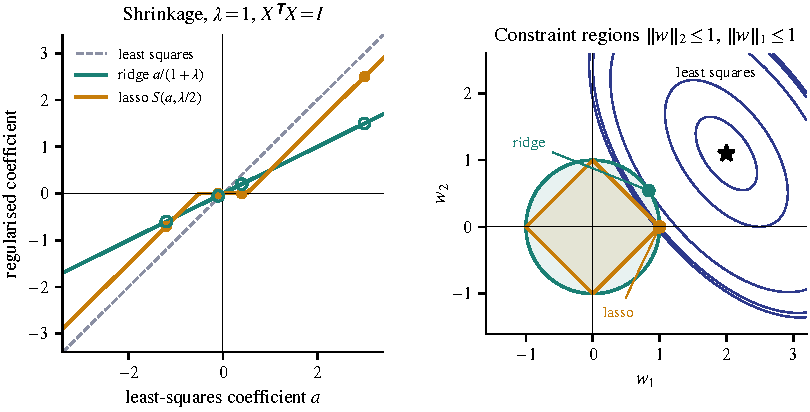
\includegraphics[width=0.94\linewidth]{figures/n8_shrinkage.pdf}
\caption{Left: for an orthonormal design, ridge multiplies each least-squares coefficient by $1/(1+\lambda)$, the lasso
moves it towards zero by $\lambda/2$ and sets it to zero inside $[-\lambda/2, \lambda/2]$; the markers (filled: lasso,
open: ridge) are part~(b) of the worked example in Section~\ref{sec:soft}. Right: the constrained form. Contours of the squared error (indigo) grow from the
least-squares point until they touch the constraint region; the $L_2$ disc is touched at a generic point $(0.84, 0.54)$,
the $L_1$ diamond at its corner $(1, 0)$, where $w_2 = 0$ exactly.}
\label{fig:shrinkage}
\end{figure}

\subsection{Why exact zeros: the geometry}\label{sec:lassogeom}

With the norms of Note~1, Section~6, $\norm{\w}_1 = \sum_j |w_j|$ and $\norm{\w}_2^2 = \sum_j w_j^2$, minimising
$\norm{X\w - \y}^2 + \lambda\norm{\w}_1$ is equivalent to minimising $\norm{X\w - \y}^2$ subject to
$\norm{\w}_1 \le t$ for a suitable budget $t$ (each $\lambda$ corresponds to some $t$, by Lagrange multipliers; the
same holds for ridge with $\norm{\w}_2^2 \le t$). The solution is where the growing elliptical contours of the squared
error first touch the constraint region (Figure~\ref{fig:shrinkage}, right). The $L_2$ ball is round, and the contact
point is generically off the axes: both weights non-zero. The $L_1$ ball is a diamond (the $L_1$ unit ball of Note~5,
Section~5; in $d$ dimensions a \emph{cross-polytope}) whose corners lie on the axes and stick out. In two dimensions a
typical ellipse often touches it first at a corner, where one coordinate is exactly zero (on the edges between corners
both coordinates are non-zero). In $d$ dimensions the contact is often at a corner or on a low-dimensional face --- in
three dimensions an edge of the octahedron, where one coordinate is zero --- so several coordinates vanish. The $L_1$
ball has ever more corners and low-dimensional faces as $d$ grows, which is the geometric intuition for why lasso
solutions are typically sparse; how sparse they
are in a given problem depends on $\lambda$, on the correlations between the features and on the signal.

\subsection{Coordinate descent}\label{sec:cd}

With several features, minimise over one coordinate at a time, keeping the others fixed. For coordinate $j$, the
other features contribute a fixed prediction, and what $w_j$ must explain is the \emph{partial residual}
$\vr^{(j)} = \y_c - \sum_{k \ne j} w_k\vect{f}_k$, where $\vect{f}_k$ denotes column $k$ of $X_c$
(Section~\ref{sec:centring}). This is exactly the one-dimensional problem of Section~\ref{sec:soft}. With the full
residual $\vr = \y_c - X_c\w$ we have $\vr^{(j)} = \vr + w_j\vect{f}_j$, hence
\[
  w_j \leftarrow \frac{\soft(\rho_j, \lambda/2)}{c_j}, \qquad \rho_j = \vect{f}_j\T\vr^{(j)} = \vect{f}_j\T\vr + c_j w_j,
  \qquad c_j = \norm{\vect{f}_j}^2 .
\]
Keeping $\vr$ up to date after every change, $\vr \leftarrow \vr -
\vect{f}_j(w_j^{\text{new}} - w_j^{\text{old}})$, makes each coordinate update cost $O(n)$. Each update can only decrease
the convex objective, and cycling through the coordinates converges to the lasso solution~\cite{friedman2010}. At the
solution, every zero coefficient satisfies $|\vect{f}_j\T\vr| \le \lambda/2$ and every non-zero one
$\vect{f}_j\T\vr = \frac{\lambda}{2}\operatorname{sign}(w_j)$: the correlation of each active feature with the residual
is exactly at the threshold.

\begin{algorithm}[!tbp]
\caption{Lasso (and elastic net) by cyclic coordinate descent}
\label{alg:cd}
\begin{algorithmic}[1]
\Require $X \in \R^{n \times d}$, $\y$, penalty $\lambda > 0$, optional $\lambda_2 \ge 0$ (default $0$), tolerance $\epsilon$
\Ensure $(\hat b, \hat{\w})$ minimising $\norm{\y - b\vect{1} - X\w}^2 + \lambda\norm{\w}_1 + \lambda_2\norm{\w}_2^2$
(penalties on the standardised weights if the columns are standardised; $\lambda_2 = 0$ is the lasso)
\State centre (and usually standardise, by $\sigma_j$) $X$ and $\y$ as in Algorithm~\ref{alg:ridge}, giving $X_c$, $\y_c$
\State $\w \gets \vect{0}$ (or the solution for a nearby $\lambda$: \emph{warm start}); \ $\vr \gets \y_c - X_c\w$
\State $c_j \gets \norm{\vect{f}_j}^2$ for $j = 1, \dots, d$ \Comment{columns $\vect{f}_j$ of $X_c$; $O(nd)$, once}
\Repeat
  \For{$j = 1, \dots, d$}
    \State $\rho_j \gets \vect{f}_j\T\vr + c_j w_j$ \Comment{correlation with the partial residual, $O(n)$}
    \State $w^{\text{new}} \gets \soft(\rho_j, \lambda/2)/(c_j + \lambda_2)$ \Comment{soft threshold \eqref{eq:soft}}
    \State $\vr \gets \vr - \vect{f}_j\,(w^{\text{new}} - w_j)$; \ $w_j \gets w^{\text{new}}$ \Comment{$O(n)$; skip if unchanged}
  \EndFor
\Until{no $w_j$ changed by more than $\epsilon$ during the sweep}
\State if the columns were standardised: $w_j \gets w_j/\sigma_j$ for each $j$ \Comment{back to original units}
\State $\hat b \gets \bar y - \w\T\bar{\x}$
\State \Return $(\hat b, \w)$
\end{algorithmic}
\end{algorithm}

\begin{worked}{coordinate descent by hand}
Fit the lasso with $\lambda = 4$ (threshold $\lambda/2 = 2$) to the detector data of Section~\ref{sec:centring}. The
features are already centred, $c_1 = 10$, $c_2 = 4$, and $\y_c = \y - 4 = (-3, -2, 0, 1, 4)$. Start from $\w = (0, 0)$,
so $\vr = \y_c$.
\begin{enumerate}[label=\arabic*.,leftmargin=1.6em]
\item $j = 1$: $\rho_1 = \vect{f}_1\T\vr + 10 \cdot 0 = 6 + 2 + 0 + 1 + 8 = 17$, so $w_1 = \soft(17, 2)/10 = 15/10 = 1.5$.
Update $\vr \gets \vr - 1.5\,\vect{f}_1 = (0, -0.5, 0, -0.5, 1)$.
\item $j = 2$: $\rho_2 = \vect{f}_2\T\vr + 4 \cdot 0 = 0 + 0.5 + 0 + 0 + 1 = 1.5$. Since $|1.5| \le 2$, $w_2 = 0$: the second
feature is switched off and $\vr$ does not change.
\item Second sweep: $\rho_1 = \vect{f}_1\T\vr + 10 \cdot 1.5 = 2 + 15 = 17$ again, so $w_1 = 1.5$; $\rho_2 = 1.5$ again,
so $w_2 = 0$. Nothing changed: converged.
\end{enumerate}
The lasso solution is $\hat{\w} = (1.5, 0)$ with $\hat b = 4$, compared with least squares $(1.667, 0.333)$ and ridge
with the same $\lambda = 4$, $(X\T X + 4I)^{-1}X\T\y_c = \begin{psmallmatrix} 14 & 1 \\ 1 & 8 \end{psmallmatrix}^{-1}
\begin{psmallmatrix} 17 \\ 3 \end{psmallmatrix} = (1.198, 0.225)$ (here $X\T\y_c = X\T\y$ because the columns are centred). The optimality conditions hold: for the active
feature $\vect{f}_1\T\vr = 2 = \lambda/2$, for the inactive one $|\vect{f}_2\T\vr| = 1.5 \le 2$.
\end{worked}

\begin{runtime}{lasso by coordinate descent (Algorithm~\ref{alg:cd})}
One sweep over all $d$ coordinates costs $O(nd)$: each coordinate needs one dot product with the residual and one
residual update, both $O(n)$. The number of sweeps $T$ is typically tens to a few hundred, so training costs $O(Tnd)$,
with no $d^3$ term. Memory: the data, $O(nd)$, plus $O(n)$ for the residual and $O(d)$ for the weights. Large savings
come from \emph{warm starts} along a decreasing sequence of $\lambda$ (each solution is a good start for the next) and
from sweeping mostly over the currently non-zero coordinates; computing a whole path then costs little more than one
fit~\cite{friedman2010}. With a sparse $X$ each sweep costs only $O(\mathrm{nnz}(X))$, the number of non-zero
entries. The elastic-net term $\lambda_2$ only changes a denominator and leaves all costs unchanged. The updates are
sequential over $j$, so GPUs help little; the method is fast because each step is cheap.
\emph{Prediction}: $O(k)$ per query, where $k$ is the number of non-zero coefficients --- a sparse model is also a cheap model.
\end{runtime}

\subsection{Elastic net and regularisation paths}\label{sec:paths}

The \emph{elastic net} adds both penalties, $\lambda_1\norm{\w}_1 + \lambda_2\norm{\w}_2^2$, keeping the sparsity of the
lasso while behaving better with groups of correlated features~\cite{zou2005}: the lasso tends to pick one member of a
correlated group more or less arbitrarily (the two thermometers again), the $L_2$ part spreads the weight over the
group. Coordinate descent handles it with a one-line change, $w_j \leftarrow \soft(\rho_j, \lambda_1/2)/(c_j + \lambda_2)$:
the extra term $\lambda_2 w_j^2$ adds $\lambda_2$ to the coefficient $c_j$ of $w_j^2$ in the one-dimensional problem
(Algorithm~\ref{alg:cd} with $\lambda = \lambda_1$).

\begin{worked}{lasso and elastic net on the two thermometers}
Take data set A of the thermometer example (Section~\ref{sec:unstable}), whose inputs and targets are already centred,
with $\lambda_1 = 2$ (threshold $1$). The lasso by coordinate descent from $\w = (0, 0)$: $\rho_1 = \vect{f}_1\T\y = 19.8$,
so $w_1 = \soft(19.8, 1)/10 = 1.88$. The new residual is $\vr = \y - 1.88\,\vect{f}_1 = (-0.34, 0.08, 0.12, 0.14)$ and
$\rho_2 = \vect{f}_2\T\vr = 0.996 \le 1$, so $w_2 = 0$. A second sweep changes nothing: the lasso answer is $(1.88, 0)$.
All the weight goes to the first thermometer, although the data cannot tell the two apart (data set B gives $(1.90, 0)$).
Adding $\lambda_2 = 1$ turns the second thermometer back on: coordinate descent now needs many sweeps, because the two
coordinates are strongly coupled, and converges to the elastic-net solution $(0.921, 0.885)$ --- two similar weights,
like ridge, whose sum $1.81$ is shrunk somewhat below the well-determined total $w_1 + w_2 \approx 2$. Neither weight is exactly zero, but in a
larger problem the irrelevant features would still be removed by the $L_1$ part.
\end{worked}

Figure~\ref{fig:paths} follows the coefficients of eight correlated features, of which three matter, as $\lambda$ grows.
Ridge shrinks all of them smoothly and none reaches zero. The lasso removes the irrelevant ones first: eight non-zero
coefficients at $\lambda = 1$, five at $\lambda = 10$, four at $25$ and only the three true ones at $\lambda = 100$. Which
$\lambda$ to use is decided on validation data (Note~4, Section~7).

\begin{figure}[!htbp]
\centering
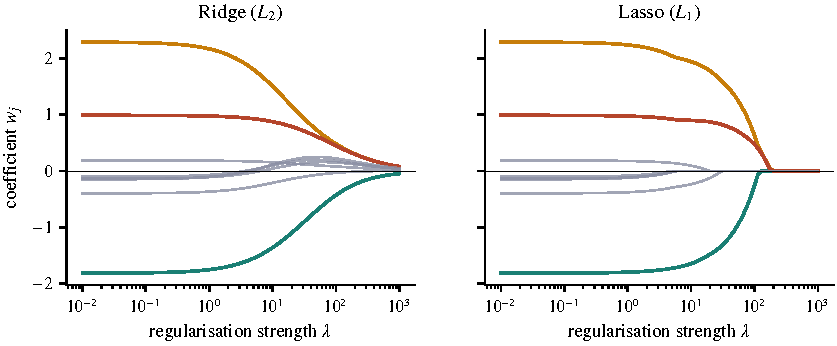
\includegraphics[width=\linewidth]{figures/reg_paths.pdf}
\caption{Regularisation paths for $n = 60$ examples with eight standardised, correlated features; coloured lines are
the three features with non-zero true weights $(2, -1.5, 1)$, grey lines the five irrelevant ones.}
\label{fig:paths}
\end{figure}

\section{The Bayesian reading}\label{sec:bayesian}

Model the targets as $y_i = \w\T\xt_i + \varepsilon_i$ with independent Gaussian noise $\varepsilon_i \sim
\Normal(0, \sigma^2)$, and put a prior $p(\w)$ on the weights. The derivation of the \emph{maximum a posteriori} (MAP)
estimate takes four steps.
\begin{enumerate}[label=\arabic*.,leftmargin=1.6em]
\item Bayes' rule (Note~2, Section~1): $p(\w \mid \text{data}) = p(\text{data} \mid \w)\,p(\w)/p(\text{data})$, and the
denominator does not depend on $\w$.
\item Likelihood (as in Note~2, Section~3): by independence, $p(\text{data} \mid \w) = \prod_i \frac{1}{\sqrt{2\pi}\sigma}
\exp\!\big(-(y_i - \w\T\xt_i)^2/(2\sigma^2)\big)$.
\item Take $-\log$, which turns the product into a sum and maximisation into minimisation:
\[
  -\log p(\w \mid \text{data}) = \frac{1}{2\sigma^2}\norm{\Xt\w - \y}^2 - \log p(\w) + \text{const}.
\]
\item Multiply by $2\sigma^2$, which does not move the minimiser:
\[
  \hat{\w}_{\mathrm{MAP}} = \argmin_{\w}\ \norm{\Xt\w - \y}^2 - 2\sigma^2\log p(\w) .
\]
\end{enumerate}
A flat prior gives back least squares. A Gaussian prior $w_j \sim \Normal(0, \tau^2)$ on the weights (and a flat one on
the bias) gives $-\log p(\w) = \sum_{j=1}^d w_j^2/(2\tau^2) + $ const, hence
\[
  \hat{\w}_{\mathrm{MAP}} = \argmin_{\w}\ \norm{\Xt\w - \y}^2 + \frac{\sigma^2}{\tau^2}\sum_{j=1}^d w_j^2 :
  \qquad \text{ridge with } \lambda = \sigma^2/\tau^2 .
\]
Strong regularisation means a narrow prior relative to the noise. A Laplace prior $p(w_j) = \frac{1}{2\beta}
e^{-|w_j|/\beta}$ gives $-2\sigma^2\log p(\w) = (2\sigma^2/\beta)\sum_{j=1}^d |w_j| + $ const: the lasso with
$\lambda = 2\sigma^2/\beta$. Its sharp peak at zero is what produces exact zeros. A regulariser is a prior belief about
the parameters, made explicit.

\begin{worked}{MAP estimate of the cart velocity}
For the cart, suppose the position measurements have noise variance $\sigma^2 = 0.5$\,cm$^2$, and that before the
experiment we believed the velocity to be small: $w \sim \Normal(0, \tau^2)$ with $\tau^2 = 0.25$\,(cm/s)$^2$. Then
$\lambda = \sigma^2/\tau^2 = 2$ and the MAP slope is the ridge slope $22/(10 + 2) = 1.833$\,cm/s, with
$\hat b = 5 - 2 \times 1.833 = 1.333$\,cm. To check this directly, write the log-posterior of the slope up to a
constant. Because the bias is not penalised, for every $w$ its best value is $b = \bar y - w\bar x$
(Section~\ref{sec:line}); substituting it turns each residual $y_i - b - wx_i$ into $(y_i - \bar y) - w(x_i - \bar x)$, so
the centred data enter:
\[
  \ell(w) = -\frac{1}{2\sigma^2}\sum_i \big((y_i - \bar y) - w(x_i - \bar x)\big)^2 - \frac{w^2}{2\tau^2}
          = -(50 - 44w + 10w^2) - 2w^2 ,
\]
using $\sum (y_i - \bar y)^2 = 50$, $\sum (x_i - \bar x)(y_i - \bar y) = 22$, $\sum (x_i - \bar x)^2 = 10$ and $2\sigma^2 = 1$.
Setting $\ell'(w) = 44 - 20w - 4w = 0$ gives $w = 44/24 = 1.833$. Numerically, $\ell(1.7) = -9.88$, $\ell(1.833) = -9.667$,
$\ell(2.0) = -10.00$ and, at the least-squares slope, $\ell(2.2) = -11.28$: the prior pulls the estimate towards zero. Since
$\ell$ is quadratic, the posterior is Gaussian: a log-density $-aw^2 + kw + \text{const}$ is that of a Gaussian with
variance $1/(2a)$ (compare the exponent $-(w - \mu)^2/(2v)$, whose $w^2$ coefficient is $1/(2v)$). Here $a = 10 + 2 = 12$,
so the variance is $1/24 = 0.0417$; in general $a = (S_{xx} + \lambda)/(2\sigma^2)$, giving $\sigma^2/(S_{xx} + \lambda)$.
This is a standard deviation of $0.20$\,cm/s --- an error bar that the point estimate alone does not give. With a Laplace prior of
scale $\beta = 0.25$ instead, $\lambda = 2\sigma^2/\beta = 4$ and the MAP slope is the lasso value $\soft(22, 2)/10 = 2.0$
of the soft-thresholding example in Section~\ref{sec:soft}.
\end{worked}

\begin{modern}{linear probes read out what a network knows}
Ridge regression is a standard instrument for asking what information a trained network's activations contain: record
the activation vector $\x$ of some layer for many inputs, regress a quantity of interest on it, and evaluate on held-out
inputs. Applied to the activations of large language models reading names of places, historical figures, works of art and
news headlines, such
\emph{linear probes} predict latitude, longitude and dates well, suggesting that these quantities are represented along
roughly linear directions~\cite{gurnee2024}. The activation vectors have thousands of components, comparable to the
number of labelled examples in many probing studies, so the regularisation of Section~\ref{sec:ridge} is not optional. A
good probe fit shows that information is \emph{present}, not that the network \emph{uses} it.
\end{modern}

\begin{physics}{discovering equations by sparse regression}
To find the law $\dot{\vect{z}} = F(\vect{z})$ behind a measured trajectory, build a large library of candidate terms ---
$1, z_1, z_2, z_1^2, z_1 z_2, \sin z_1, \dots$ --- evaluated along the data, and regress the measured derivatives on it with
a sparsity-promoting method. Most coefficients vanish, and the few that remain form a readable equation. With this approach
(``sparse identification of nonlinear dynamics'') the Lorenz equations were recovered from simulated
trajectories~\cite{brunton2016}; the original work used sequentially thresholded least squares, and the lasso of
Section~\ref{sec:lasso} is a common alternative.
Linear regression on non-linear features, with a sparsity prior playing the role of Occam's razor, becomes a tool for
model discovery.
\end{physics}

\section{Algorithms at a glance}\label{sec:glance}

Table~\ref{tab:costs} collects the algorithms of this note: $n$ examples, $d$ features, mini-batch size $n'$, $T$
iterations or sweeps, $k$ non-zero lasso coefficients, $\kappa$ the condition number of $X\T X$; the boxes above use
$p = d + 1$, which is $\approx d$ in these leading terms.

\begin{table}[!tbp]
\centering\small
\caption{Costs of the regression algorithms of this note (leading terms; $p = d + 1 \approx d$).}
\label{tab:costs}
\setlength{\tabcolsep}{4pt}
\begin{tabular}{L{3.4cm}L{3.7cm}L{2.1cm}L{5.1cm}}
\toprule
Algorithm & Training time & Memory & Use when \\
\midrule
Simple regression (Alg.~\ref{alg:simple}) & $O(n)$ & $O(1)$ & one input; hand calculations \\
Normal equations (Alg.~\ref{alg:normal}) & $O(nd^2 + d^3)$ & $O(d^2)$, streaming & $d$ up to a few thousand, well-conditioned features \\
QR (Alg.~\ref{alg:qr}) & $O(nd^2)$ & $O(nd)$ & moderate $d$, ill-conditioned but full-rank $X$ \\
SVD, \texttt{lstsq} (Alg.~\ref{alg:svdls}) & $O(nd\min(n,d))$, larger constant & $O(nd)$ & default for moderate $d$; rank-deficient $X$, $d \ge n$ \\
Gradient descent, mini-batch SGD (Alg.~\ref{alg:gd}) & $O(nd)$ per epoch, $T$ epochs & $O(n'd)$ & huge $n$ or $d$, sparse data, streaming \\
Conjugate gradient (LSQR) & $O(nd)$ per iteration, at most $d + 1$ iterations & $O(n + d)$ extra & large sparse $X$, faster than GD when ill-conditioned \\
Ridge (Alg.~\ref{alg:ridge}) & $O(nd^2 + d^3)$; $O(d\min(n,d))$ per extra $\lambda$; dual $O(n^2 d + n^3)$ & $O(d^2)$ or $O(n^2)$ & collinear features, $d \ge n$, many $\lambda$ to compare \\
Lasso / elastic net, coordinate descent (Alg.~\ref{alg:cd}) & $O(nd)$ per sweep, $T$ sweeps & $O(nd)$ & feature selection, interpretable sparse models \\
\bottomrule
\end{tabular}
\end{table}

Prediction costs $O(d)$ per query for every method ($O(k)$ for a sparse lasso model). Direct methods are exact and
predictable; iterative ones scale, but their iteration counts grow with $\kappa$, which standardising reduces.

\Needspace{10\baselineskip}
\begin{keyidea}[Summary]
Linear regression predicts $\w\T\x + b$; a column of ones absorbs the bias, centring separates it again
($\hat b = \bar y - \hat{\w}\T\bar{\x}$). Least squares sets the gradient $2\Xt\T(\Xt\w - \y)$ to zero: the normal equations,
an orthogonal projection, the maximum-likelihood fit under Gaussian noise (slope $S_{xy}/S_{xx}$ for one input). Solve by
Cholesky, QR/SVD or gradient descent. Collinear features make it unstable, $d \ge n$ undetermined. Ridge
($\lambda\norm{\w}^2$) shrinks each SVD direction by $s_j^2/(s_j^2 + \lambda)$; the lasso ($\lambda\norm{\w}_1$)
soft-thresholds and selects features, by coordinate descent. Both are MAP estimates, under Gaussian and Laplace priors.
\end{keyidea}

\begin{questions}
\begin{conceptual}
\item Linear regression is ``linear'' in what? Which of these can be fitted by linear least squares, possibly after
transforming variables: $y = a + bx + cx^2$; $y = a\sin x + b\cos x$; $y = a e^{bx}$ ($y > 0$); $y = a/(1 + e^{-b(x-c)})$,
with $a$, $b$, $c$ all unknown?
\item Explain the bias trick in words. Why does the bias get its own treatment in ridge regression and the lasso, and
what would go wrong with the predictions if all targets were shifted by $+100$ and the bias were penalised?
\item Explain, without formulas, why the least-squares residual vector is orthogonal to every column of the design
matrix, and what ``the fitted values are a projection of the targets'' means.
\item Two thermometers that read almost the same temperature are both used as features. Explain why the individual
least-squares weights are unreliable even though the predictions are good. Which combination of the two weights is well
determined, and which is not?
\item What happens to least squares when there are more parameters than examples ($d + 1 > n$)? Is the solution unique,
what does \texttt{np.linalg.lstsq} return, and how does adding a ridge penalty change the situation?
\item Why should one not compute $(\Xt\T\Xt)^{-1}$ explicitly? What advantage does a QR or SVD solver have over the
normal equations, in terms of the condition number?
\item Compare ridge and lasso: which one produces coefficients that are exactly zero, and why? Give one explanation using
the one-dimensional formulas and one using the shape of the constraint regions.
\item A feature is a length. Explain what happens to its ridge coefficient, and to how strongly it is penalised, if the
length is recorded in millimetres instead of metres, with the same $\lambda$. What practical rule follows?
\item Describe what the ridge and lasso estimates become as $\lambda \to 0$ and as $\lambda \to \infty$. Relate the two
limits to underfitting, overfitting, bias and variance (Note~4).
\item In the Bayesian reading, which prior gives ridge and which gives the lasso? If the measurement noise variance
$\sigma^2$ doubles while the prior stays the same, how does the equivalent $\lambda$ change, and why does that make sense?
\item The period $T$ of a pendulum is measured for several lengths $\ell$. Which linear regression, on which transformed
variables, estimates the exponent $\alpha$ in $T \propto \ell^{\alpha}$? Least squares on the transformed variables
assumes Gaussian noise of constant size on $\log T$: what does that mean for the errors of the measured periods $T$
themselves?
\item Which algorithm of Table~\ref{tab:costs} would you choose (a) for $n = 10^8$ examples and $d = 50$ features
stored on disk, when you need the exact least-squares answer after a single pass over the disk, (b) for the same data
when an approximate answer is enough and you want to update the model as new examples arrive, (c) for a ridge or lasso
fit with $n = 500$ and $d = 10^5$? Why?
\item Gradient descent on a least-squares problem diverges. What is the likely cause, what sets the largest allowed
learning rate, and how does standardising the features help?
\item The lasso is applied to a data set containing three almost identical features. What will it typically do with
them, and how does the elastic net change this behaviour?
\item A linear probe trained on the activations of a neural network predicts the temperature of a simulated system with
$R^2 = 0.95$ on held-out data. What does this show, and what does it not show?
\item Why is the $L_2$ penalty also called ``weight decay''? Explain qualitatively, in terms of which directions of
the weight space are fitted quickly and which slowly, why stopping gradient descent early, starting from
$\w = \vect{0}$, has an effect similar to a ridge penalty.
\item Why does one sweep of lasso coordinate descent cost only $O(nd)$, with no $d^3$ term? Why do warm starts along a
decreasing sequence of $\lambda$ values make a whole regularisation path cheap?
\item A model reaches $R^2 = 0.99$ on its training data. Why is this not enough to conclude that it will predict well on
new data? What would you check, and could the training $R^2$ become negative for least squares with a bias?
\end{conceptual}

\begin{calculations}
\item Fit a line to the points $(x, y) = (1, 2), (2, 3), (3, 5), (4, 6)$: compute $\bar x$, $\bar y$, $S_{xy}$, $S_{xx}$,
the slope and the intercept. Compute the four residuals, check that they sum to zero, and compute $R^2$.
\item For $J(b, w) = \sum_i (y_i - b - wx_i)^2$, write $\partial J/\partial b$ and $\partial J/\partial w$. Evaluate both
at $(b, w) = (0, 1)$ for the data of B1, take one gradient-descent step with $\eta = 0.01$, and check that $J$ decreases
(here use the sum $J$, not the mean loss $L$ of Section~\ref{sec:computing}).
\item For centred data with $\sum_i x_i^2 = 8$ and $\sum_i x_i y_i = 12$, compute the ridge slope for $\lambda = 0, 4, 12$
and the corresponding shrinkage factors. For which $\lambda$ is the slope half of the least-squares slope?
\item For an orthonormal design ($X\T X = I$) the least-squares coefficients are $\vect{a} = (2.4, -0.6, 1.1, -3.0)$.
Compute the lasso and the ridge coefficients for $\lambda = 2$. How many features does each method keep?
\item Centred features give $X\T X = \begin{psmallmatrix} 4 & 2 \\ 2 & 2 \end{psmallmatrix}$ and $X\T\y =
(6, 4)\T$. Solve the normal equations, then the ridge equations with $\lambda = 2$. If the uncentred feature means were
$\bar{\x} = (1, 2)$ and $\bar y = 3$, what are the two intercepts?
\item The noise variance is $\sigma^2 = 0.2$ and the prior on a single centred slope is Gaussian with mean $0$ and
variance $\tau^2 = 0.05$; the data give
$\sum x_i^2 = 16$ and $\sum x_i y_i = 10$. Compute the equivalent $\lambda$, the least-squares slope and the MAP slope. Repeat
with a Laplace prior of scale $\beta = 0.2$ instead.
\item The singular values of a centred design matrix are $(10, 3, 1, 0.1)$. Compute the ridge shrinkage factor of each
direction and the effective number of parameters for $\lambda = 1$. (Remember that the factors use $s_j^2$.)
\end{calculations}

\begin{derivations}
\item Expand $\norm{\Xt\w - \y}^2$, derive its gradient and the normal equations, and show that with a column of ones the
residuals sum to zero. Show that for one input the slope is $\widehat{\Cov}(x, y)/\widehat{\Var}(x)$.
\item Derive the ridge solution, including the matrix $\Ic$. Show that $\Xt\T\Xt + \lambda\Ic$ is positive definite
for every $\lambda > 0$, even when $d > n$. (Consider $\vect{v}\T(\Xt\T\Xt + \lambda\Ic)\vect{v}$ separately for $\vect{v}$ with
and without non-zero weight components.)
\item Using the SVD, show that the ridge fitted values are $\sum_j \vect{u}_j s_j^2/(s_j^2 + \lambda)\, \vect{u}_j\T\y$ for
centred data, and that the coefficients are $\sum_j \vect{v}_j s_j/(s_j^2 + \lambda)\,\vect{u}_j\T\y$.
\item Show that the minimiser of $(w - a)^2 + \lambda|w|$ is $\operatorname{sign}(a)\max(|a| - \lambda/2, 0)$, treating the
cases $w > 0$, $w < 0$ and $w = 0$, and explain why the $L_2$ penalty never produces exact zeros.
\item Prove the identity $(X\T X + \lambda I_d)^{-1}X\T = X\T(XX\T + \lambda I_n)^{-1}$ (multiply both sides by suitable
matrices). Conclude that the ridge solution can be written $\hat{\w} = X\T\vect{\alpha}$ with
$\vect{\alpha} = (XX\T + \lambda I)^{-1}\y$, and compare the costs of the two forms when $d \gg n$.
\end{derivations}

\begin{programming}
\item Implement Algorithms~\ref{alg:normal}, \ref{alg:qr} and~\ref{alg:gd} in numpy and compare their results and
running times for $n = 10^4$, $d = 100$. Then make two columns nearly collinear ($\vect{f}_2 = \vect{f}_1 + 10^{-6}\times$noise) and
compare the accuracy of the normal equations with that of QR.
\item Reproduce Figure~\ref{fig:collinear}. Then fit least squares with gradient descent from $\w = \vect{0}$ and stop after
$k$ steps: compare the spread of the estimates with that of ridge. Which $k$ behaves like $\lambda = 3$?
\item Implement Algorithm~\ref{alg:cd}. Check it on the hand calculation of Section~\ref{sec:cd} ($\lambda = 4$ must give $(1.5, 0)$), then
reproduce the lasso panel of Figure~\ref{fig:paths} with warm starts and choose $\lambda$ by 5-fold cross-validation.
Optionally, recover the two terms of a simulated damped oscillator $\ddot z = -4z - 0.3\dot z$ from the library
$\{1, z, \dot z, z^2, z\dot z, \dot z^2\}$, as in the physics box of Section~\ref{sec:bayesian}.
\end{programming}
\end{questions}

\paragraph{Further reading} Hastie, Tibshirani and Friedman~\cite{hastie2009}, chapter~3; Bishop~\cite{bishop2006},
chapter~3; for sparsity, Hastie, Tibshirani and Wainwright~\cite{hastie2015}.

\begin{thebibliography}{99}\small
\bibitem{bishop2006} C.~M. Bishop, \emph{Pattern Recognition and Machine Learning}, Springer (2006).
\bibitem{brunton2016} S.~L. Brunton, J.~L. Proctor and J.~N. Kutz, Discovering governing equations from data by sparse identification of nonlinear dynamical systems, \emph{Proc.\ Natl.\ Acad.\ Sci.\ USA} 113, 3932--3937 (2016).
\bibitem{friedman2010} J.~Friedman, T.~Hastie and R.~Tibshirani, Regularization paths for generalized linear models via coordinate descent, \emph{J.\ Stat.\ Softw.} 33(1), 1--22 (2010).
\bibitem{gurnee2024} W.~Gurnee and M.~Tegmark, Language models represent space and time, \emph{ICLR} (2024).
\bibitem{hastie2009} T.~Hastie, R.~Tibshirani and J.~Friedman, \emph{The Elements of Statistical Learning}, 2nd ed., Springer (2009).
\bibitem{hastie2015} T.~Hastie, R.~Tibshirani and M.~Wainwright, \emph{Statistical Learning with Sparsity: The Lasso and Generalizations}, CRC Press (2015).
\bibitem{hoerl1970} A.~E. Hoerl and R.~W. Kennard, Ridge regression: biased estimation for nonorthogonal problems, \emph{Technometrics} 12, 55--67 (1970).
\bibitem{nocedal2006} J.~Nocedal and S.~J. Wright, \emph{Numerical Optimization}, 2nd ed., Springer (2006).
\bibitem{tibshirani1996} R.~Tibshirani, Regression shrinkage and selection via the lasso, \emph{J.\ R.\ Stat.\ Soc.\ B} 58, 267--288 (1996).
\bibitem{zou2005} H.~Zou and T.~Hastie, Regularization and variable selection via the elastic net, \emph{J.\ R.\ Stat.\ Soc.\ B} 67, 301--320 (2005).
\end{thebibliography}

\SourceNote
\end{document}
